\documentclass[11pt, a4paper]{article}

% Paquetes esenciales
\usepackage[utf8]{inputenc}
\usepackage[english]{babel} % Cambia a ngerman si escribirás en alemán
\usepackage{geometry}
\geometry{a4paper, margin=2cm} % Márgenes de 2cm para aprovechar el espacio
\usepackage{graphicx} % Para insertar imágenes
\usepackage{booktabs} % Para tablas más profesionales
\usepackage{array}
\usepackage{pdflscape} % Por si necesitas poner la tabla en horizontal
\usepackage{hyperref} % Para enlaces clickeables

% Configuración de la tabla para que el texto se ajuste a las celdas
\newcolumntype{P}[1]{>{\raggedright\arraybackslash}p{#1}}

\title{\textbf{Failure Modes and Effects Analysis (FMEA)\\Scissor Jack}}
\author{Joan Sebastian Uruchima Castro \\ \small TU Dortmund}
\date{\today}

\begin{document}

\maketitle

\section{Product Definition}
% Aquí va la descripción clara e inequívoca de la gata mecánica.
The analyzed product is a mechanical scissor jack, which is a portable lifting device commonly used in the automotive industry for vehicle maintenance or tire changes. Its main purpose is to lift heavy loads vertically in a safe manner. This is achieved by converting the rotational input motion applied to a central lead screw into a linear vertical lifting force through a folding joint mechanism. 

% Ejemplo de cómo insertar tu imagen
\begin{figure}[h!]
    \centering
    % Sube tu imagen a Overleaf y cambia 'nombre_de_tu_imagen.jpg' por el archivo real
    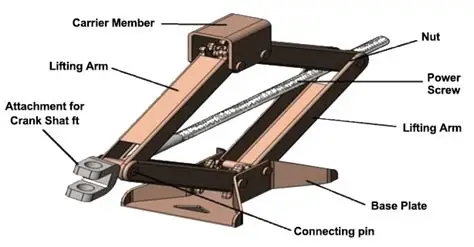
\includegraphics[width=0.5\textwidth]{Scissor Jack.png} 
    \caption{Main components of a mechanical scissor jack \cite{jack_image}.}
    \label{fig:scissor_jack}
\end{figure}

\section{System Decomposition and Boundaries}
To perform a structured Failure Modes and Effects Analysis (FMEA), the mechanical scissor jack has been divided into three subsystems. The function tree shows the hierarchical structure of the components (see Figure \ref{fig:function_tree}). The primary functions of these subsystems are described as follows:

\begin{itemize}
    \item \textbf{Structural Subsystem:} Responsible for providing a stable interface between the ground and vehicle load, ensuring that the system remains upright and aligned during operation.
    \item \textbf{Transmission Subsystem:} Responsible for receiving the rotational input from the user and converting it into a horizontal linear force via the lead screw mechanism.
    \item \textbf{Lifting Subsystem:} Acts as the kinematic linkage that transforms the horizontal force from the transmission into the required vertical displacement to elevate the vehicle.
\end{itemize}

\textbf{System Boundaries and FMEA Scope:} While the entire system is described above, this FMEA will focus on the critical component of the Transmission Subsystem: the Power Screw. External elements, the remaining subsystems, and other transmission components (such as the nut and crank attachment) are considered outside the scope and are assumed to behave nominally.

\textbf{Environmental and Operational Conditions:} The mechanism is intended to work in severe and highly variable conditions. It must be able to support high static compressive loads in operation and deal with the dynamic friction created during cranking. Environmentally, the jack is typically used outdoors. Therefore, the components are exposed to moisture, extreme temperature variations, dirt, and corrosive road salts, all of which significantly accelerate material degradation and affect lubrication.

% ---- AQUÍ VA TU DIAGRAMA DE ÁRBOL ----
\begin{figure}[h!]
    \centering
    % Cambia 'tu_diagrama.png' por el nombre del archivo que exportes de Draw.io
    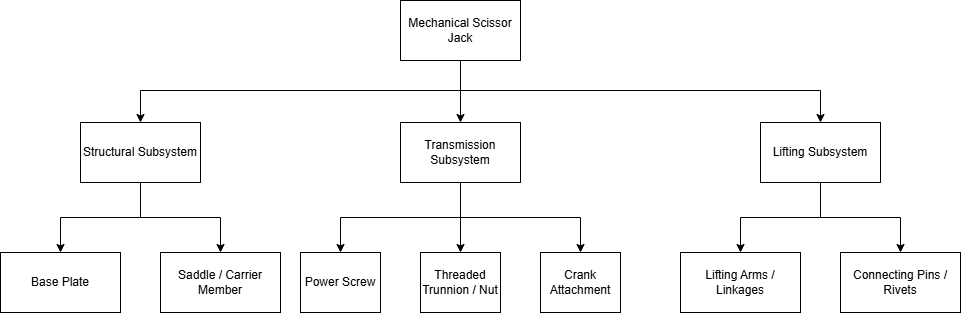
\includegraphics[width=1\textwidth]{Tree diagram.png} 
    \caption{Function tree illustrating the system decomposition of the mechanical scissor jack.}
    \label{fig:function_tree}
\end{figure}
% ---------------------------------------
\section{FMEA Table}

\begin{table}[htbp]
    \centering
    \caption{FMEA Worksheet focusing on the Power Screw (Transmission Subsystem) of the Scissor Jack.}
    \vspace{0.2cm}
    
    % Mantiene la tabla al 95% del ancho de la página para dejar márgenes limpios
    \resizebox{0.95\textwidth}{!}{
        \renewcommand{\arraystretch}{1.5} % Espacio vertical cómodo
        
        \begin{tabular}{|P{1.2cm}|P{1.6cm}|P{1.8cm}|P{1.8cm}|c|P{1.8cm}|c|P{1.6cm}|P{1.6cm}|c|c|P{2.0cm}|}
        \hline
        
        \textbf{Item} & 
        \textbf{Function} & 
        \textbf{Potential \newline Failure \newline Mode} & 
        \textbf{Potential \newline Effects \newline of Failure} &  
        \textbf{SEV} & 
        \textbf{Potential \newline Causes \newline of Failure} & 
        \textbf{OCC} & 
        \textbf{Current \newline Design \newline Controls \newline (Prev.)} & 
        \textbf{Current \newline Design \newline Controls \newline (Detec.)} & 
        \textbf{DET} & 
        \textbf{RPN} & 
        \textbf{Recom- \newline mended \newline Action(s)} \\ \hline
        
        % MODO DE FALLO 1: Desgaste / Fricción (Tribológico)
        % Usamos multirow para combinar las celdas verticalmente
        \multirow{Power \newline Screw} & {Convert rotational input to linear force} & 
        Thread stripping or extreme wear & 
        Loss of load capacity, sudden jack collapse & 
        9 & 
        High friction from inadequate lubrication, cyclic material fatigue & 
        3 & 
        Hardened steel selection (ISO 683) \cite{iso683}, safety factor in thread design & 
        Visual inspection before use & 
        4 & 
        108 & 
        Apply permanent warning label for periodic lubrication \\ \cline{3-12} % La línea solo va de la columna 3 a la 12
        
        % MODO DE FALLO 2: Sobrecarga / Pandeo (Estructural)
        % Dejamos las dos primeras celdas vacías (& &) porque ya están abarcadas por el multirow de arriba
        & & 
        Shaft yielding (bending) or buckling & 
        Mechanism binds, load shifts or cannot be lowered safely & 
        8 & 
        Overloading beyond rated capacity, off-axis loading by user & 
        2 & 
        Diameter sizing for buckling resistance (DIN 4114) \cite{din4114} & 
        User feels extreme resis- \newline tance during cranking & 
        5 & 
        80 & 
        Implement a shear pin in the crank handle to fail before the screw buckles \\ \cline{3-12}
        
        % MODO DE FALLO 3: Corrosión (Ambiental/Químico)
        & & 
        Clogging due to corrosion and debris & 
        Mechanism jams completely (user stranded, no sudden collapse) & 
        5 & 
        Exposure to moisture, dirt, and road salts & 
        5 & 
        Zinc plating (ISO 2081) \cite{iso2081} and factory applied grease & 
        Obvious visual rust, stiffness without load & 
        2 & 
        50 & 
        Design a protective rubber boot or self-cleaning thread profile \\ \hline
        
        \end{tabular}
    }
    \label{tab:fmea}
\end{table}

\section{Conclusions and Recommendations}

The quantitative analysis of the FMEA worksheet shows that the most critical vulnerability of the transmission subsystem is the tribological wear (thread stripping) of the power screw. This failure mode produced the highest Risk Priority Number (RPN = 108) and maximum Severity rating (SEV = 9) due to the catastrophic nature of a sudden jack collapse. The main recommendation to reduce this risk is to treat the root cause (high friction) by adding a permanent maintenance label to ensure periodical lubrication. 

Moreover, the structural buckling has a lower RPN (80) but its high severity (SEV = 8) needs significant design attention. It is strongly recommended to have some fail safe mechanism like a shear pin in the external crank handle. This ensures that the system yields safely under user-induced overload before the primary power screw can permanently deform. Finally, environmental corrosion (RPN = 50) is considered to be lower priority due to its high visual detectability which can be reduced thru the inclusion of a protective rubber boot in future design iterations.

\vspace{1em} % Espacio antes de las referencias

% Sección de referencias para citar tu imagen
\begin{thebibliography}{9}

\bibitem{jack_image} 
ATO.com (2023). 
\textit{What is a Scissor Jack?}. 
Available at: \url{https://www.ato.com/what-is-a-scissor-jack} (Accessed: 17 August 2026).

\bibitem{iso683}
International Organization for Standardization (2018).
\textit{ISO 683-1:2018 Heat-treatable steels, alloy steels and free-cutting steels}. Geneva, Switzerland.

\bibitem{din4114}
Deutsches Institut für Normung (1952).
\textit{DIN 4114: Steel structures; stability cases (buckling, overturning, bulging)}. Berlin, Germany.

\bibitem{iso2081}
International Organization for Standardization (2025).
\textit{ISO 2081:2025 Metallic and other inorganic coatings — Electroplated coatings on iron and steel using zinc treated with solutions containing chromium (VI)}. Geneva, Switzerland.

\end{thebibliography}

\end{document}